% Options for packages loaded elsewhere
\PassOptionsToPackage{unicode}{hyperref}
\PassOptionsToPackage{hyphens}{url}
%
\documentclass[
  10pt,
  ignorenonframetext,
  aspectratio=169,
  notheorems]{beamer}
\usepackage{pgfpages}
\setbeamertemplate{caption}[numbered]
\setbeamertemplate{caption label separator}{: }
\setbeamercolor{caption name}{fg=normal text.fg}
\beamertemplatenavigationsymbolsempty
% Prevent slide breaks in the middle of a paragraph
\widowpenalties 1 10000
\raggedbottom
\setbeamertemplate{part page}{
  \centering
  \begin{beamercolorbox}[sep=16pt,center]{part title}
    \usebeamerfont{part title}\insertpart\par
  \end{beamercolorbox}
}
\setbeamertemplate{section page}{
  \centering
  \begin{beamercolorbox}[sep=12pt,center]{part title}
    \usebeamerfont{section title}\insertsection\par
  \end{beamercolorbox}
}
\setbeamertemplate{subsection page}{
  \centering
  \begin{beamercolorbox}[sep=8pt,center]{part title}
    \usebeamerfont{subsection title}\insertsubsection\par
  \end{beamercolorbox}
}
\AtBeginPart{
  \frame{\partpage}
}
\AtBeginSection{
  \ifbibliography
  \else
    \frame{\sectionpage}
  \fi
}
\AtBeginSubsection{
  \frame{\subsectionpage}
}

\usepackage{amsmath,amssymb}
\usepackage{iftex}
\ifPDFTeX
  \usepackage[T1]{fontenc}
  \usepackage[utf8]{inputenc}
  \usepackage{textcomp} % provide euro and other symbols
\else % if luatex or xetex
  \usepackage{unicode-math}
  \defaultfontfeatures{Scale=MatchLowercase}
  \defaultfontfeatures[\rmfamily]{Ligatures=TeX,Scale=1}
\fi
\usepackage{lmodern}
\usetheme[]{Berlin}
\ifPDFTeX\else  
    % xetex/luatex font selection
\fi
% Use upquote if available, for straight quotes in verbatim environments
\IfFileExists{upquote.sty}{\usepackage{upquote}}{}
\IfFileExists{microtype.sty}{% use microtype if available
  \usepackage[]{microtype}
  \UseMicrotypeSet[protrusion]{basicmath} % disable protrusion for tt fonts
}{}
\makeatletter
\@ifundefined{KOMAClassName}{% if non-KOMA class
  \IfFileExists{parskip.sty}{%
    \usepackage{parskip}
  }{% else
    \setlength{\parindent}{0pt}
    \setlength{\parskip}{6pt plus 2pt minus 1pt}}
}{% if KOMA class
  \KOMAoptions{parskip=half}}
\makeatother
\usepackage{xcolor}
\newif\ifbibliography
\setlength{\emergencystretch}{3em} % prevent overfull lines
\setcounter{secnumdepth}{-\maxdimen} % remove section numbering


\providecommand{\tightlist}{%
  \setlength{\itemsep}{0pt}\setlength{\parskip}{0pt}}\usepackage{longtable,booktabs,array}
\usepackage{calc} % for calculating minipage widths
\usepackage{caption}
% Make caption package work with longtable
\makeatletter
\def\fnum@table{\tablename~\thetable}
\makeatother
\usepackage{graphicx}
\makeatletter
\def\maxwidth{\ifdim\Gin@nat@width>\linewidth\linewidth\else\Gin@nat@width\fi}
\def\maxheight{\ifdim\Gin@nat@height>\textheight\textheight\else\Gin@nat@height\fi}
\makeatother
% Scale images if necessary, so that they will not overflow the page
% margins by default, and it is still possible to overwrite the defaults
% using explicit options in \includegraphics[width, height, ...]{}
\setkeys{Gin}{width=\maxwidth,height=\maxheight,keepaspectratio}
% Set default figure placement to htbp
\makeatletter
\def\fps@figure{htbp}
\makeatother
% definitions for citeproc citations
\NewDocumentCommand\citeproctext{}{}
\NewDocumentCommand\citeproc{mm}{%
  \begingroup\def\citeproctext{#2}\cite{#1}\endgroup}
\makeatletter
 % allow citations to break across lines
 \let\@cite@ofmt\@firstofone
 % avoid brackets around text for \cite:
 \def\@biblabel#1{}
 \def\@cite#1#2{{#1\if@tempswa , #2\fi}}
\makeatother
\newlength{\cslhangindent}
\setlength{\cslhangindent}{1.5em}
\newlength{\csllabelwidth}
\setlength{\csllabelwidth}{3em}
\newenvironment{CSLReferences}[2] % #1 hanging-indent, #2 entry-spacing
 {\begin{list}{}{%
  \setlength{\itemindent}{0pt}
  \setlength{\leftmargin}{0pt}
  \setlength{\parsep}{0pt}
  % turn on hanging indent if param 1 is 1
  \ifodd #1
   \setlength{\leftmargin}{\cslhangindent}
   \setlength{\itemindent}{-1\cslhangindent}
  \fi
  % set entry spacing
  \setlength{\itemsep}{#2\baselineskip}}}
 {\end{list}}
\usepackage{calc}
\newcommand{\CSLBlock}[1]{\hfill\break\parbox[t]{\linewidth}{\strut\ignorespaces#1\strut}}
\newcommand{\CSLLeftMargin}[1]{\parbox[t]{\csllabelwidth}{\strut#1\strut}}
\newcommand{\CSLRightInline}[1]{\parbox[t]{\linewidth - \csllabelwidth}{\strut#1\strut}}
\newcommand{\CSLIndent}[1]{\hspace{\cslhangindent}#1}

\makeatletter
\@ifpackageloaded{caption}{}{\usepackage{caption}}
\AtBeginDocument{%
\ifdefined\contentsname
  \renewcommand*\contentsname{Table of contents}
\else
  \newcommand\contentsname{Table of contents}
\fi
\ifdefined\listfigurename
  \renewcommand*\listfigurename{List of Figures}
\else
  \newcommand\listfigurename{List of Figures}
\fi
\ifdefined\listtablename
  \renewcommand*\listtablename{List of Tables}
\else
  \newcommand\listtablename{List of Tables}
\fi
\ifdefined\figurename
  \renewcommand*\figurename{Figure}
\else
  \newcommand\figurename{Figure}
\fi
\ifdefined\tablename
  \renewcommand*\tablename{Table}
\else
  \newcommand\tablename{Table}
\fi
}
\@ifpackageloaded{float}{}{\usepackage{float}}
\floatstyle{ruled}
\@ifundefined{c@chapter}{\newfloat{codelisting}{h}{lop}}{\newfloat{codelisting}{h}{lop}[chapter]}
\floatname{codelisting}{Listing}
\newcommand*\listoflistings{\listof{codelisting}{List of Listings}}
\makeatother
\makeatletter
\makeatother
\makeatletter
\@ifpackageloaded{caption}{}{\usepackage{caption}}
\@ifpackageloaded{subcaption}{}{\usepackage{subcaption}}
\makeatother
\ifLuaTeX
  \usepackage{selnolig}  % disable illegal ligatures
\fi
\usepackage{bookmark}

\IfFileExists{xurl.sty}{\usepackage{xurl}}{} % add URL line breaks if available
\urlstyle{same} % disable monospaced font for URLs
\hypersetup{
  pdftitle={Against Spurious Sparks − Dovelating Inflated AI Claims},
  pdfauthor={Patrick Altmeyer; Andrew M. Demetriou; Antony Bartlett; Cynthia C. S. Liem},
  hidelinks,
  pdfcreator={LaTeX via pandoc}}

\title{Against Spurious Sparks − Dovelating Inflated AI Claims}
\subtitle{ECONDAT Conference 2024\footnote<.->{Upcoming position paper
  at ICML 2024.}}
\author{Patrick Altmeyer \and Andrew M. Demetriou \and Antony
Bartlett \and Cynthia C. S. Liem}
\date{2024-05-07}
\institute{Delft University of Technology}

\begin{document}
\frame{\titlepage}

\begin{frame}{Motivation}
\phantomsection\label{motivation}
\begin{columns}[T]
\begin{column}{0.5\textwidth}
\begin{itemize}
\tightlist
\item
  \(A_1\): „It is essential to bring inflation back to target to avoid
  drifting into deflation territory.``
\item
  \(A_2\): „It is essential to bring the numbers of doves back to target
  to avoid drifting into dovelation territory.``
\end{itemize}

\begin{quote}
``They're exactly the same.''

--- Linear probe \(\widehat{cpi}=f(A)\)
\end{quote}
\end{column}

\begin{column}{0.5\textwidth}
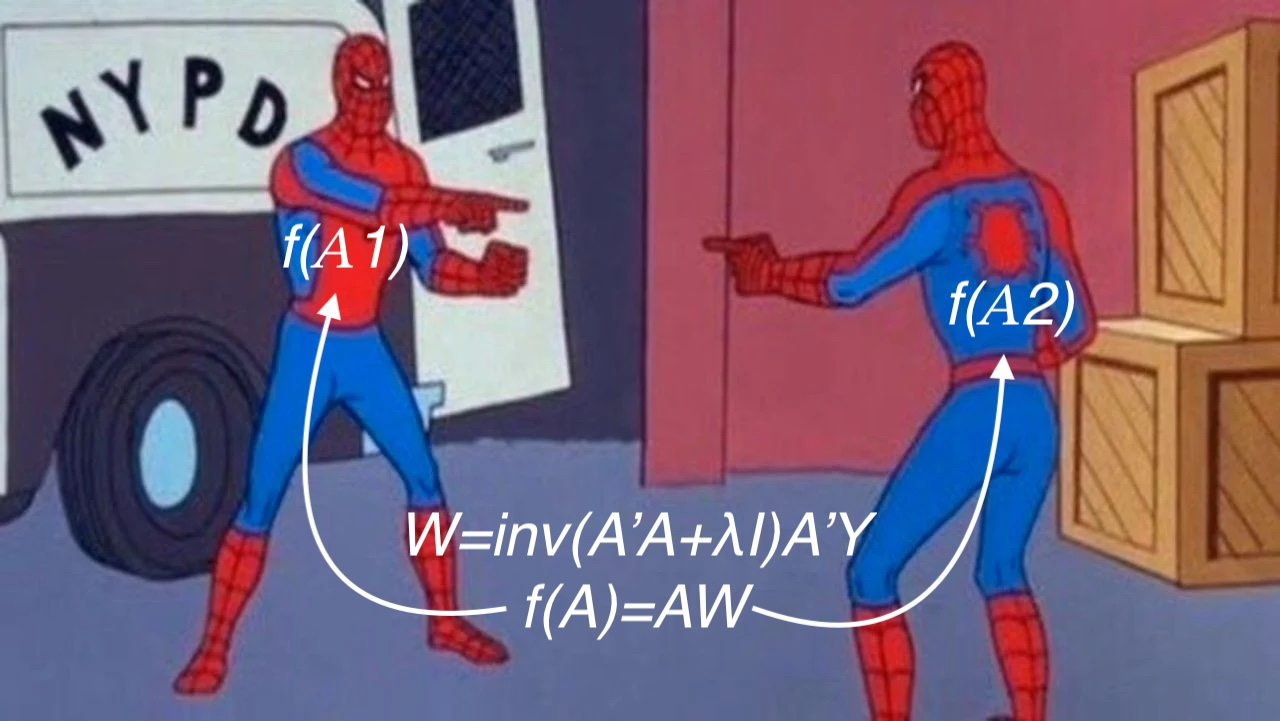
\includegraphics{www/spider.jpeg}
\end{column}
\end{columns}
\end{frame}

\begin{frame}{Position}
\phantomsection\label{position}
\begin{quote}
Current LLMs embed knowledge. They don`t „understand`` anything. They
are useful tools, but tools nonetheless.
\end{quote}

\begin{itemize}[<+->]
\tightlist
\item
  Meaningful patterns in embeddings are like doves in the sky.
\item
  Humans are prone to seek patterns and anthropomorphize.
\item
  Observed `sparks' of Artificial General Intelligence are spurious.
\item
  The academic community should exercise extra caution.
\item
  Publishing incentives need to be adjusted.
\end{itemize}
\end{frame}

\begin{frame}{Outline}
\phantomsection\label{outline}
\begin{itemize}[<+->]
\tightlist
\item
  \textbf{Experiments}: We probe models of varying complexity including
  random projections, matrix decompositions, deep autoencoders and
  transformers.

  \begin{itemize}[<+->]
  \tightlist
  \item
    All of them successfully distill knowledge and yet none of them
    develop true understanding.
  \end{itemize}
\item
  \textbf{Social sciences review}: Humans are prone to seek patterns and
  anthropomorphize.
\item
  \textbf{Conclusion and outlook}: More caution at the individual level,
  and different incentives at the institutional level.
\end{itemize}
\end{frame}

\section{There! It's sentient!}\label{there-its-sentient}

\begin{frame}{There! It's sentient!}
\begin{center}

\includegraphics{www/leo.png}
\end{center}
\end{frame}

\begin{frame}{The Holy Grail}
\phantomsection\label{the-holy-grail}
Achievement of Artificial General Intelligence (AGI) has become a grand
challenge, and in some cases, an explicit business goal.

\begin{columns}[T]
\begin{column}{0.5\textwidth}
\begin{block}{Definition}
\phantomsection\label{definition}
The definition of AGI itself is not as clear-cut or consistent:

\begin{itemize}
\tightlist
\item
  (loosely) a phenomenon contrasting with `narrow AI' systems, that were
  trained for specific tasks (Goertzel 2014).
\end{itemize}
\end{block}
\end{column}

\begin{column}{0.5\textwidth}
\begin{block}{Practice}
\phantomsection\label{practice}
Researchers have sought to show that AI models generalize to different
(and possibly unseen) tasks or show performance considered `surprising'
to humans.

\begin{itemize}
\tightlist
\item
  For example, Google DeepMind claimed their AlphaGeometry model (Trinh
  et al. 2024) reached a `milestone' towards AGI.
\end{itemize}
\end{block}
\end{column}
\end{columns}
\end{frame}

\begin{frame}{A Perfect Storm}
\phantomsection\label{a-perfect-storm}
Recent developments in the field have created a `perfect storm' for
inflated claims:

\begin{itemize}[<+->]
\tightlist
\item
  Early sharing of preprints and code.
\item
  Volume of publishable work has exploded.
\item
  Social media influencers start playing a role in article discovery and
  citeability (Weissburg et al. 2024).
\item
  Complexity is increasing because it is incentivized (Birhane et al.
  2022).
\end{itemize}
\end{frame}

\begin{frame}{``Not Mere Stochastic Parrots''}
\phantomsection\label{not-mere-stochastic-parrots}
\begin{itemize}
\tightlist
\item
  We consider a recently viral work (Gurnee and Tegmark 2023a), in which
  claims about the learning of world models by LLMs were made.

  \begin{itemize}
  \tightlist
  \item
    Linear probes (ridge regression) were successfully used to predict
    geographical locations from LLM embeddings.
  \end{itemize}
\item
  Claims on
  \href{https://twitter.com/tegmark/status/1709572469978231063}{X} that
  this indicates that LLMs are not mere `stochastic parrots' (Bender et
  al. 2021).
\item
  Reactions on X seemed to largely exhibit excitement and surprise at
  the authors' findings.
\end{itemize}
\end{frame}

\section{On the unsurprising nature of latent
embeddings}\label{on-the-unsurprising-nature-of-latent-embeddings}

\begin{frame}{Are Neural Networks Born with World Models?}
\phantomsection\label{are-neural-networks-born-with-world-models}
\begin{columns}[T]
\begin{column}{0.6\textwidth}
\begin{itemize}
\tightlist
\item
  Llama-2 model tested in Gurnee and Tegmark (2023b) has ingested huge
  amounts of publicly available data (Touvron et al. 2023).

  \begin{itemize}
  \tightlist
  \item
    Geographical locations are literally in the training data:
    e.g.~Wikipedia \href{https://en.wikipedia.org/wiki/London}{article}
    for ``London''.
  \item
    Where would this information be encoded if not in the embedding
    space \(\mathcal{A}\)? Is it surprising that
    \(A_{\text{LDN}}=enc(\text{"London"}) \not\!\perp\!\!\!\perp (\text{lat}_{\text{LDN}},\text{long}_{\text{LDN}})\)?
  \end{itemize}
\item
  Figure~\ref{fig-map} shows the predicted coordinates of a linear probe
  on the final-layer activations of an untrained neural network.
\end{itemize}
\end{column}

\begin{column}{0.4\textwidth}
\begin{figure}

\centering{

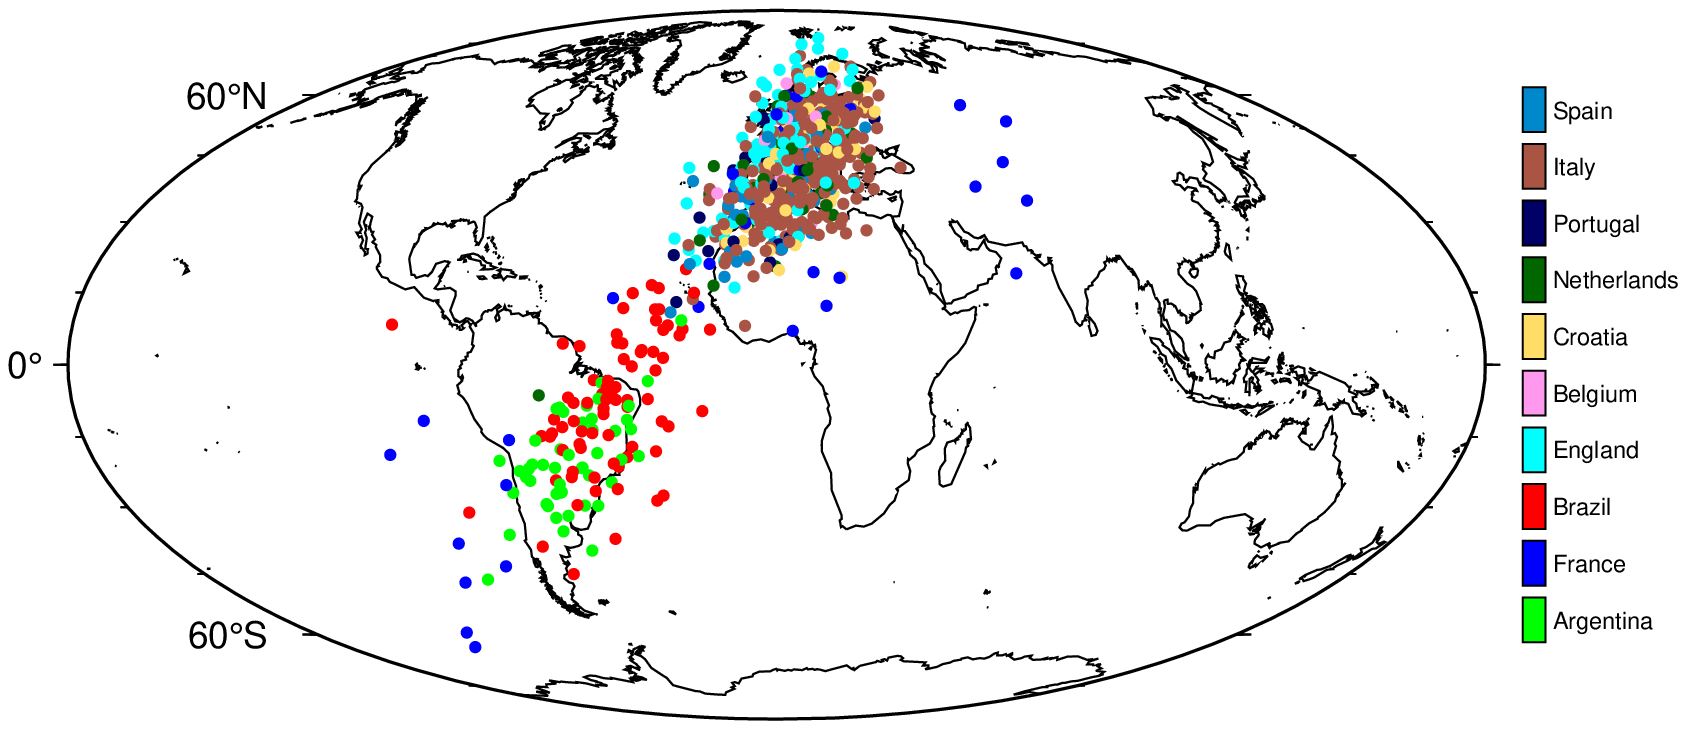
\includegraphics{www/map.png}

}

\caption{\label{fig-map}Predicted coordinate values (out-of-sample) from
a linear probe on final-layer activations of an untrained neural
network.}

\end{figure}%

\begin{itemize}
\tightlist
\item
  Model has seen noisy coordinates plus \(d\) random features.
\item
  Single hidden layer with \(h < d\) hidden units.
\end{itemize}
\end{column}
\end{columns}
\end{frame}

\begin{frame}{PCA as a Yield Curve Interpreter}
\phantomsection\label{pca-as-a-yield-curve-interpreter}
What are principal components if not model embeddings?

\begin{figure}

\centering{

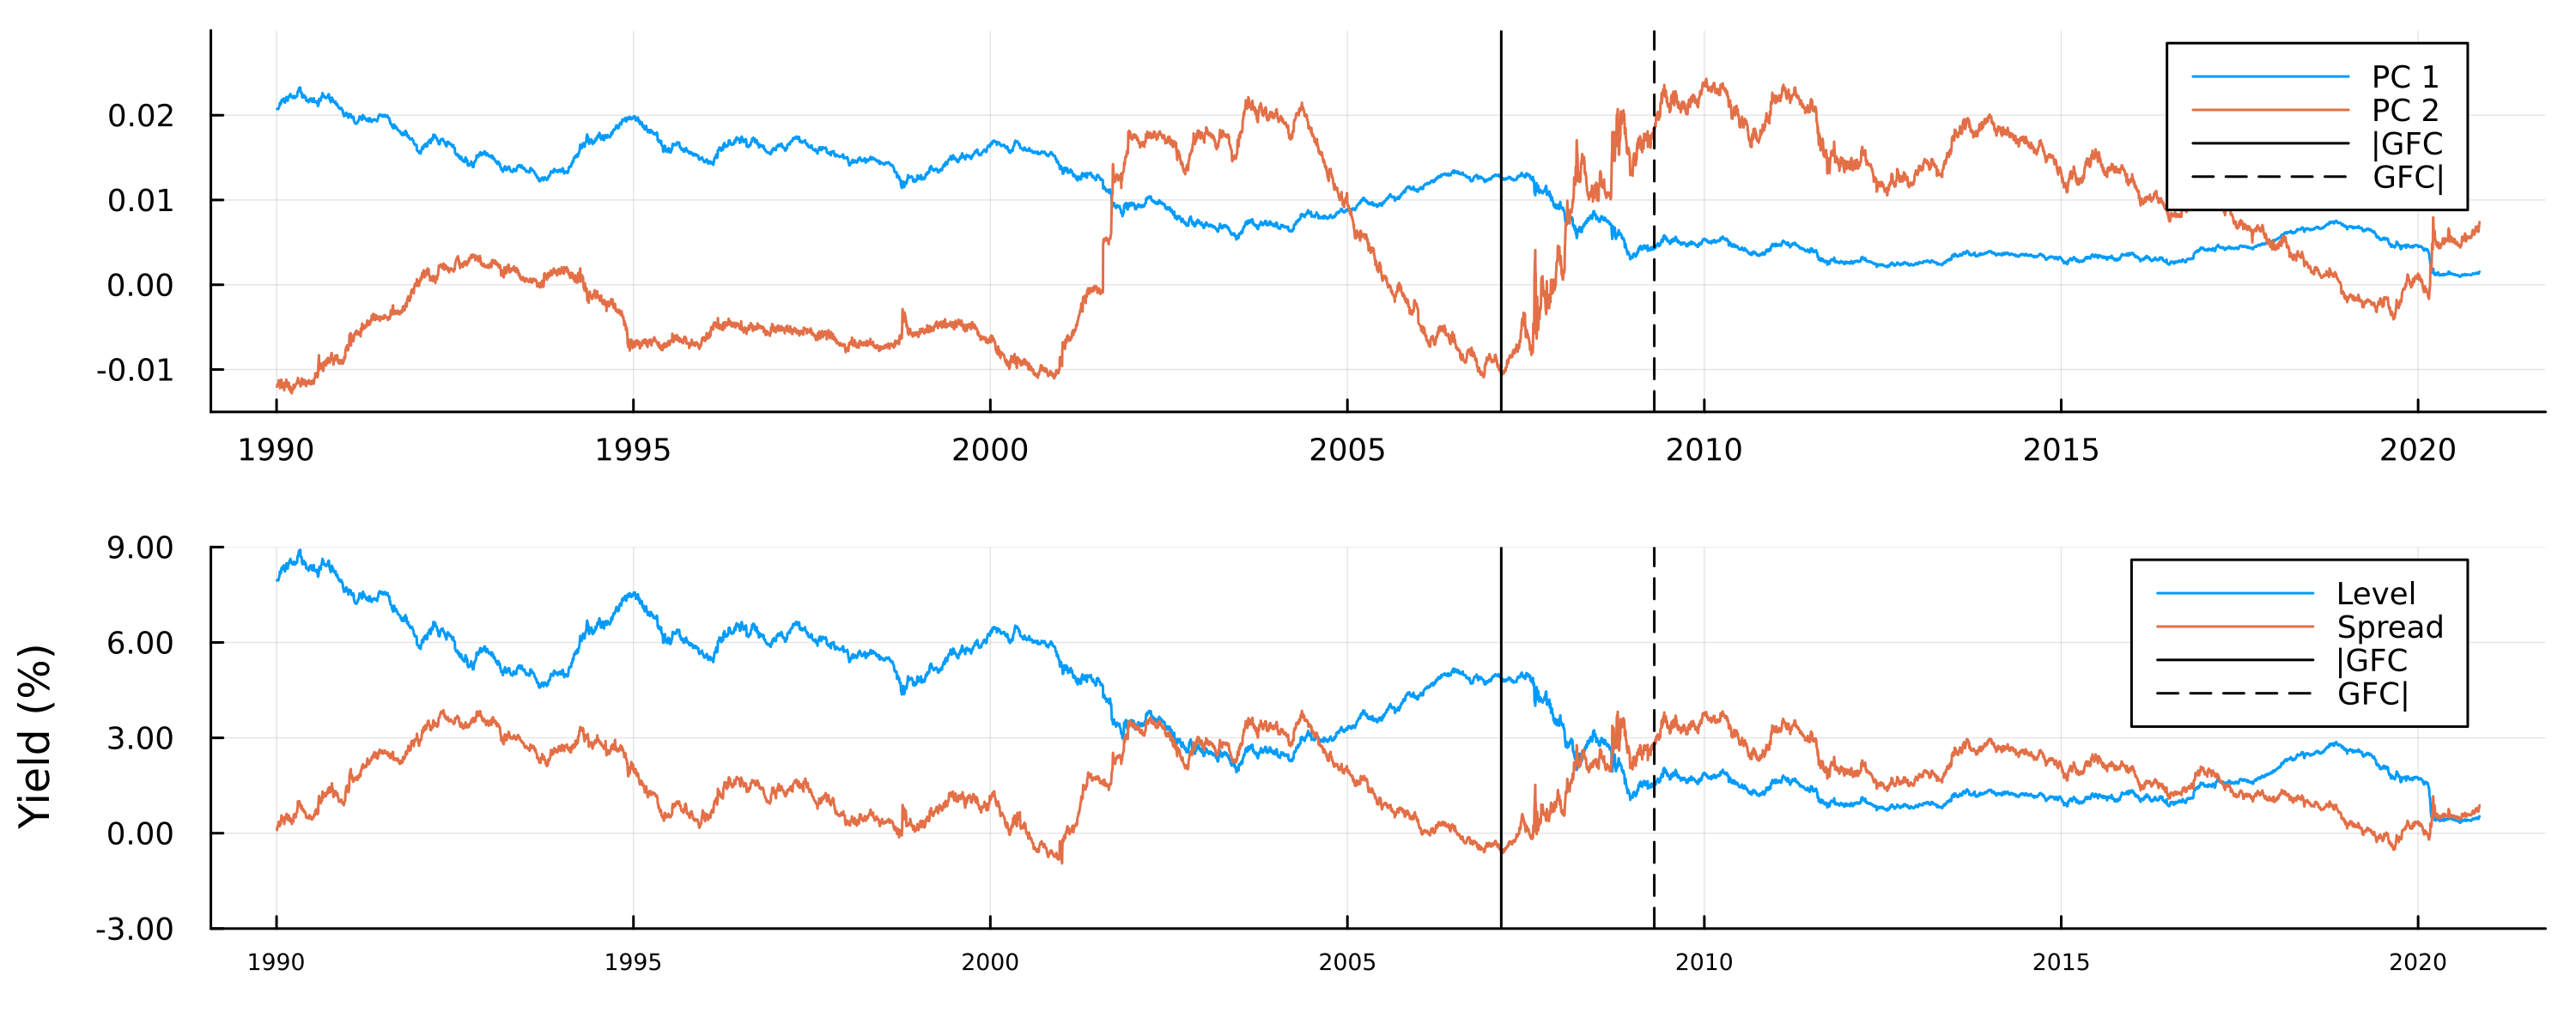
\includegraphics[width=0.8\textwidth,height=\textheight]{www/pca_yield.png}

}

\caption{\label{fig-pca}Top chart: The first two principal components of
US Treasury yields over time at daily frequency. Bottom chart: Observed
average level and 10yr-3mo spread of the yield curve. Vertical stalks
roughly indicate the onset (\textbar GFC) and the beginning of the
aftermath (GFC\textbar) of the Global Financial Crisis.}

\end{figure}%
\end{frame}

\begin{frame}{Embedding FOMC comms}
\phantomsection\label{embedding-fomc-comms}
\begin{itemize}
\tightlist
\item
  BERT-based model trained on FOMC minutes, speeches and press
  conferences to classify statements as hawkish or dovish (or neutral)
  (Shah, Paturi, and Chava 2023).
\item
  We linearly probe all layers to predict unseen economic indicators
  (CPI, PPI, UST yields).
\item
  Predictive power increases with layer depth and probes outperform
  simple AR(\(p\)) models.
\end{itemize}

\begin{figure}

\centering{

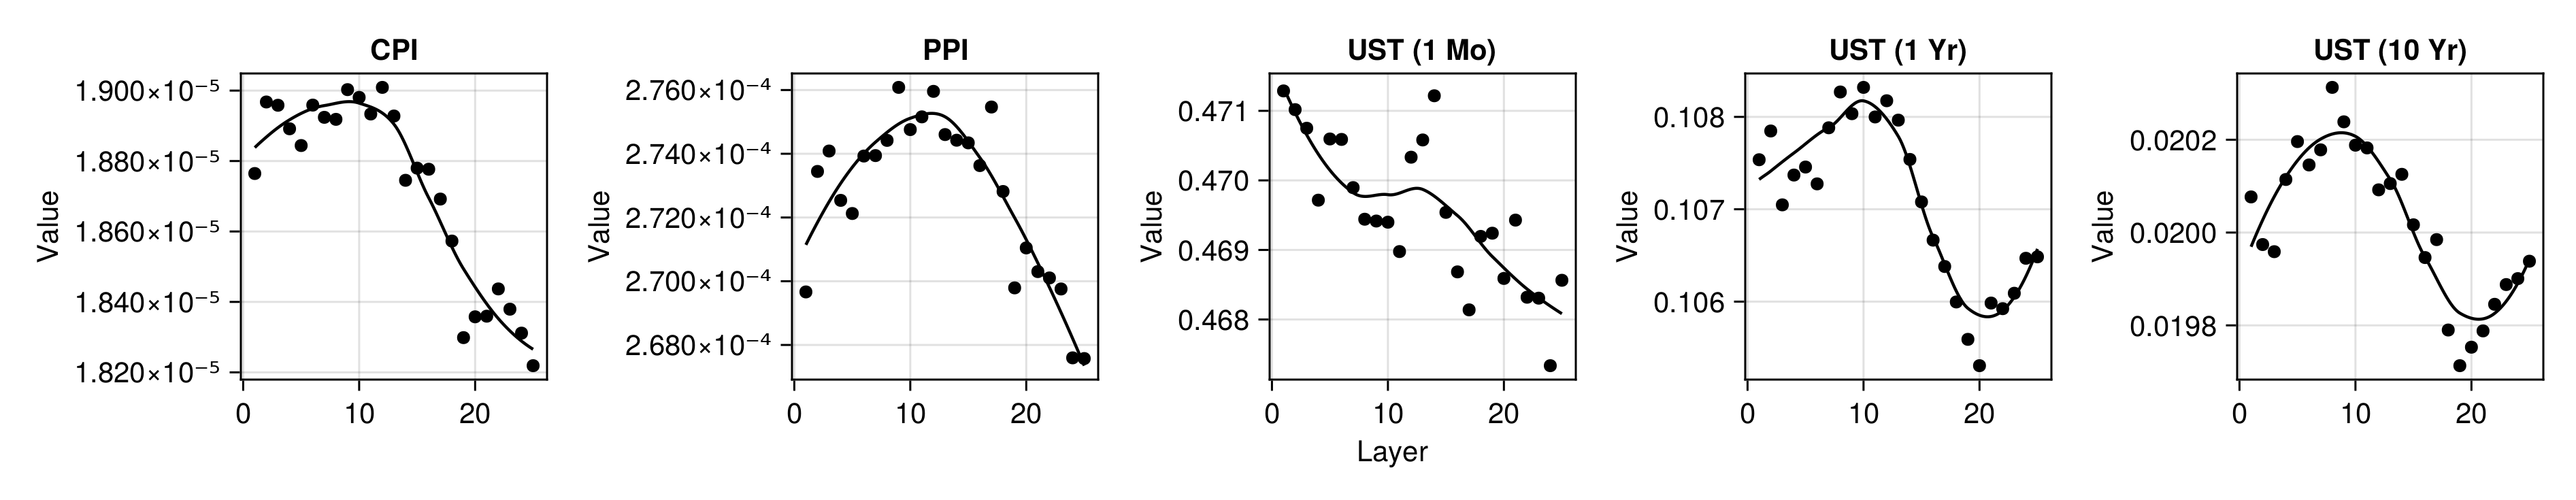
\includegraphics[width=0.8\textwidth,height=\textheight]{www/mse_pca_128.png}

}

\caption{\label{fig-mse}Out-of-sample root mean squared error (RMSE) for
the linear probe plotted against FOMC-RoBERTa's n-th layer for different
indicators.}

\end{figure}%
\end{frame}

\begin{frame}{Sparks of Economic Understanding?}
\phantomsection\label{sparks-of-economic-understanding}
\textbf{Premise}: If probe results were indicative of some intrinsic
`understanding' of the economy, then the probe should not be sensitive
to random sentences unrelated to economics.

\begin{block}{Parrot Test}
\phantomsection\label{parrot-test}
\begin{enumerate}
\tightlist
\item
  Select the best-performing probe for each economic indicator.
\item
  Predict inflation levels for real (related) and perturbed (unrelated)
  sentences.
\end{enumerate}

\begin{figure}

\centering{

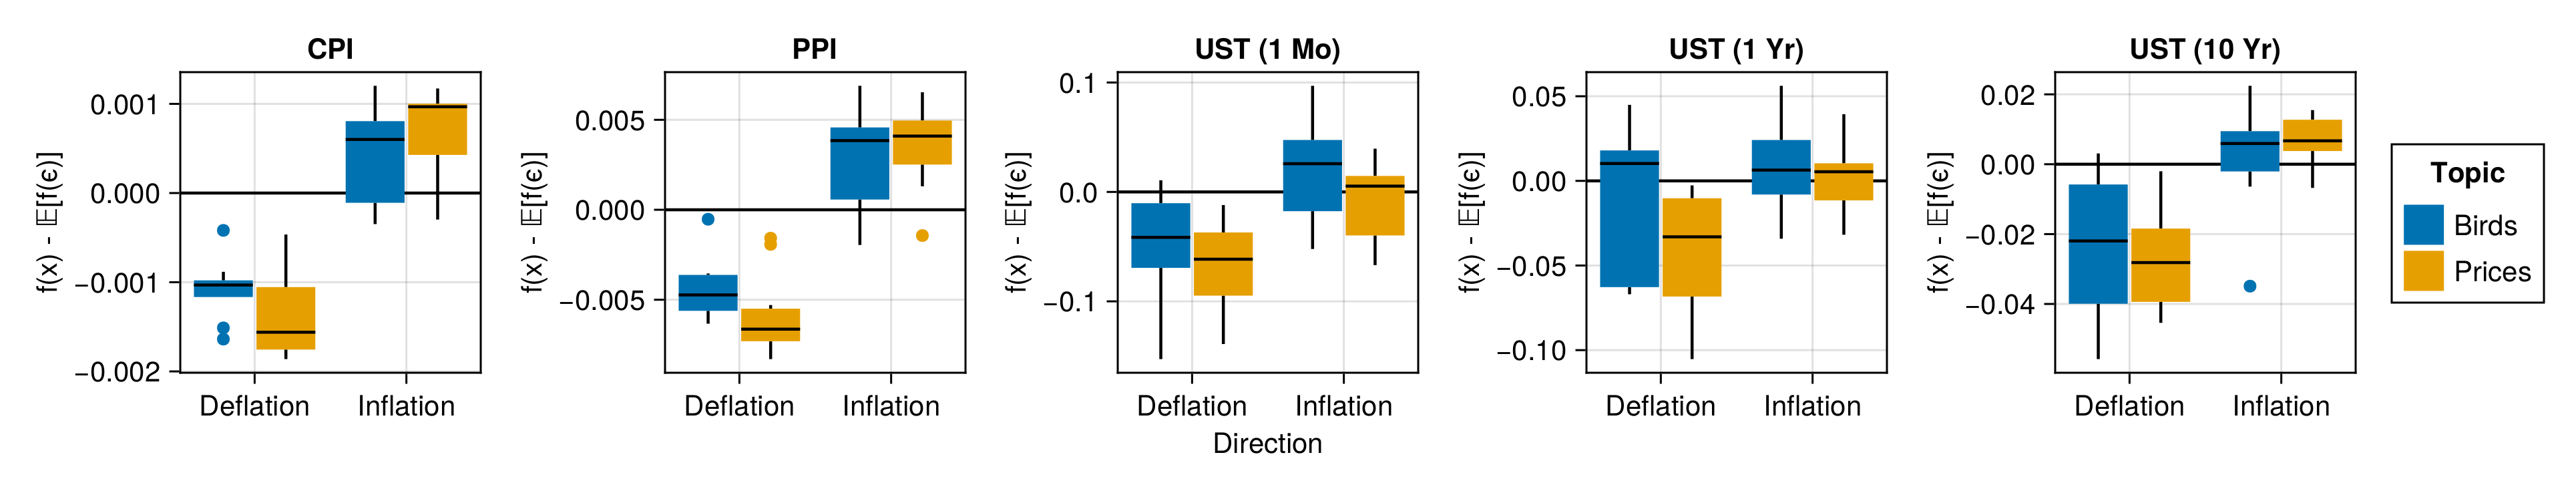
\includegraphics[width=0.8\textwidth,height=\textheight]{www/attack_all_measures.png}

}

\caption{\label{fig-attack}Probe predictions for sentences about
inflation of prices (IP), deflation of prices (DP), inflation of birds
(IB) and deflation of birds (DB). The vertical axis shows predicted
inflation levels subtracted by the average predicted value of the probe
for random noise.}

\end{figure}%

As evidenced by Figure~\ref{fig-attack}, the probe is easily fooled.
\end{block}
\end{frame}

\section{Human Proneness to
Over-Interpretation}\label{human-proneness-to-over-interpretation}

\begin{frame}{Spurious Relationships}
\phantomsection\label{spurious-relationships}
\textbf{Definiton}: Varies somewhat (Haig 2003) but distinctly implies
that the observation of correlations does not imply causation.

\begin{itemize}
\tightlist
\item
  Humans struggle to tell the difference between random and non-random
  sequences (Falk and Konold 1997).
\item
  Lack of expectation that randomness that hints towards a causal
  relationship will still appear at random.
\item
  Even experts perceive correlations of inflated magnitude (Nickerson
  1998) and causal relationships where none exist (Zgraggen et al.
  2018).
\end{itemize}
\end{frame}

\begin{frame}{Antropomorphism}
\phantomsection\label{antropomorphism}
\textbf{Definition}: Human tendency to attribute human-like
characteristics to non-human agents and/or objects.

\begin{enumerate}
\tightlist
\item
  Experience as humans is an always-readily-available template to
  interpret the world (Epley, Waytz, and Cacioppo 2007).
\item
  Motivation to avoid loneliness may lead us to anthropomorphize
  inanimate objects Waytz, Epley, and Cacioppo (2010).
\item
  Motivation to be competent may lead us anthropomorphize opaque
  technologies like LLMs Waytz, Epley, and Cacioppo (2010)
\end{enumerate}
\end{frame}

\begin{frame}{Confirmation Bias}
\phantomsection\label{confirmation-bias}
\textbf{Definition}: Favoring interpretations of evidence that support
existing beliefs or hypotheses (Nickerson 1998).

\begin{itemize}
\tightlist
\item
  Hypotheses in present-day AI research are often implicit, often framed
  simply as a system being more accurate or efficient, compared to other
  systems.

  \begin{itemize}
  \tightlist
  \item
    Failing to articulate a sufficiently strong null hypothesis leading
    to a `weak' experiment (Claesen et al. 2022).
  \end{itemize}
\item
  Individuals may place greater emphasis on evidence in support of their
  hypothesis, and lesser emphasis on evidence that opposes it (Nickerson
  1998).
\end{itemize}
\end{frame}

\begin{frame}{Conclusion and Outlook}
\phantomsection\label{conclusion-and-outlook}
\begin{itemize}
\tightlist
\item
  We call for the community to create explicit room for organized
  skepticism

  \begin{itemize}
  \tightlist
  \item
    Welcome negative results
  \item
    Encouraging replication studies.
  \item
    Move from authorship to contribution-based credit (see
    e.g.~\href{https://ieeexplore.ieee.org/stamp/stamp.jsp?tp=&arnumber=10173886}{Liem
    and Demetriou, 2023} and
    \href{https://www.bmj.com/content/315/7110/696.short}{Smith, 1997}).
  \end{itemize}
\item
  Return to the Mertonian norms (communism, universalism,
  disinterestedness, organized skepticism) (Merton et al. 1942).
\end{itemize}
\end{frame}

\section{Questions?}\label{questions}

\begin{frame}{Questions?}
With thanks to my co-authors Andrew M. Demetriou, Antony Bartlett, and
Cynthia C. S. Liem and to the audience for their attention.

\begin{center}

\includegraphics[width=0.25\textwidth,height=\textheight]{../../../../www/images/qr.png}
\end{center}
\end{frame}

\begin{frame}{References}
\phantomsection\label{references}
\phantomsection\label{refs}
\begin{CSLReferences}{1}{0}
\bibitem[\citeproctext]{ref-bender2021dangers}
Bender, Emily M, Timnit Gebru, Angelina McMillan-Major, and Shmargaret
Shmitchell. 2021. {``{On the dangers of stochastic parrots: Can language
models be too big?
\raisebox{-2pt}{\includegraphics[scale=0.1]{parrot.png}}}.''} In
\emph{Proceedings of the 2021 ACM Conference on Fairness,
Accountability, and Transparency}, 610--23.

\bibitem[\citeproctext]{ref-values_in_ML}
Birhane, Abeba, Pratyusha Kalluri, Dallas Card, William Agnew, Ravit
Dotan, and Michelle Bao. 2022. {``{The Values Encoded in Machine
Learning Research}.''} In \emph{Proceedings of the 2022 ACM Conference
on Fairness, Accountability, and Transparency (FAccT '22)}.

\bibitem[\citeproctext]{ref-claesen2022severity}
Claesen, Aline, Daniel Lakens, Noah van Dongen, et al. 2022.
{``{Severity and Crises in Science: Are We Getting It Right When We're
Right and Wrong When We're Wrong?}''}

\bibitem[\citeproctext]{ref-epley2007seeing}
Epley, Nicholas, Adam Waytz, and John T Cacioppo. 2007. {``{On seeing
human: a three-factor theory of anthropomorphism.}''}
\emph{Psychological Review} 114 (4): 864.

\bibitem[\citeproctext]{ref-falk1997making}
Falk, Ruma, and Clifford Konold. 1997. {``{Making sense of randomness:
Implicit encoding as a basis for judgment.}''} \emph{Psychological
Review} 104 (2): 301.

\bibitem[\citeproctext]{ref-goertzel2014artificial}
Goertzel, Ben. 2014. {``{Artificial general intelligence: concept, state
of the art, and future prospects}.''} \emph{Journal of Artificial
General Intelligence} 5 (1): 1.

\bibitem[\citeproctext]{ref-gurnee2023languagev2}
Gurnee, Wes, and Max Tegmark. 2023b. {``{Language Models Represent Space
and Time}.''} \emph{arXiv Preprint arXiv:2310.02207v2}.

\bibitem[\citeproctext]{ref-gurnee2023languagev1}
---------. 2023a. {``Language Models Represent Space and Time.''}
\emph{arXiv Preprint arXiv:2310.02207v1}.

\bibitem[\citeproctext]{ref-haig2003spurious}
Haig, Brian D. 2003. {``{What is a spurious correlation?}''}
\emph{Understanding Statistics: Statistical Issues in Psychology,
Education, and the Social Sciences} 2 (2): 125--32.

\bibitem[\citeproctext]{ref-merton1942science}
Merton, Robert K et al. 1942. {``{Science and technology in a democratic
order}.''} \emph{Journal of Legal and Political Sociology} 1 (1):
115--26.

\bibitem[\citeproctext]{ref-nickerson1998confirmation}
Nickerson, Raymond S. 1998. {``{Confirmation bias: A ubiquitous
phenomenon in many guises}.''} \emph{Review of General Psychology} 2
(2): 175--220.

\bibitem[\citeproctext]{ref-shah2023trillion}
Shah, Agam, Suvan Paturi, and Sudheer Chava. 2023. {``{Trillion Dollar
Words: A New Financial Dataset, Task \& Market Analysis}.''} \emph{arXiv
Preprint arXiv:2310.02207v1}. \url{https://arxiv.org/abs/2305.07972}.

\bibitem[\citeproctext]{ref-touvron2023llama}
Touvron, Hugo, Thibaut Lavril, Gautier Izacard, Xavier Martinet,
Marie-Anne Lachaux, Timothée Lacroix, Baptiste Rozière, et al. 2023.
{``{LLaMA: Open and Efficient Foundation Language Models}.''}
\url{https://arxiv.org/abs/2302.13971}.

\bibitem[\citeproctext]{ref-trinh2024geometry}
Trinh, T. H., Wu, Y., Le, and Q. V. et al. 2024. {``{Solving olympiad
geometry without human demonstrations.}''} \emph{Nature 625}, 476--82.
https://doi.org/\url{https://doi.org/10.1038/s41586-023-06747-5}.

\bibitem[\citeproctext]{ref-waytz2010social}
Waytz, Adam, Nicholas Epley, and John T Cacioppo. 2010. {``{Social
cognition unbound: Insights into anthropomorphism and
dehumanization}.''} \emph{Current Directions in Psychological Science}
19 (1): 58--62.

\bibitem[\citeproctext]{ref-weissburg2024tweets}
Weissburg, Iain Xie, Mehir Arora, Liangming Pan, and William Yang Wang.
2024. {``{Tweets to Citations: Unveiling the Impact of Social Media
Influencers on AI Research Visibility}.''} \emph{arXiv Preprint
arXiv:2401.13782}.

\bibitem[\citeproctext]{ref-zgraggen2018investigating}
Zgraggen, Emanuel, Zheguang Zhao, Robert Zeleznik, and Tim Kraska. 2018.
{``{Investigating the effect of the multiple comparisons problem in
visual analysis}.''} In \emph{Proceedings of the 2018 CHI Conference on
Human Factors in Computing Systems}, 1--12.

\end{CSLReferences}
\end{frame}

\section{Hiddens}\label{hiddens}

\begin{frame}{Autoencoders as Economic Growth Predictors}
\phantomsection\label{autoencoders-as-economic-growth-predictors}
\begin{itemize}
\tightlist
\item
  We train a neural network with a bottleneck layer to predict GDP
  growth from the yield curve.
\item
  This can be used for feature extraction and forecasting.

  \begin{itemize}
  \tightlist
  \item
    Bottle-neck layer embeddings predict spread and level of the yield
    curve.
  \end{itemize}
\end{itemize}

\begin{figure}

\centering{

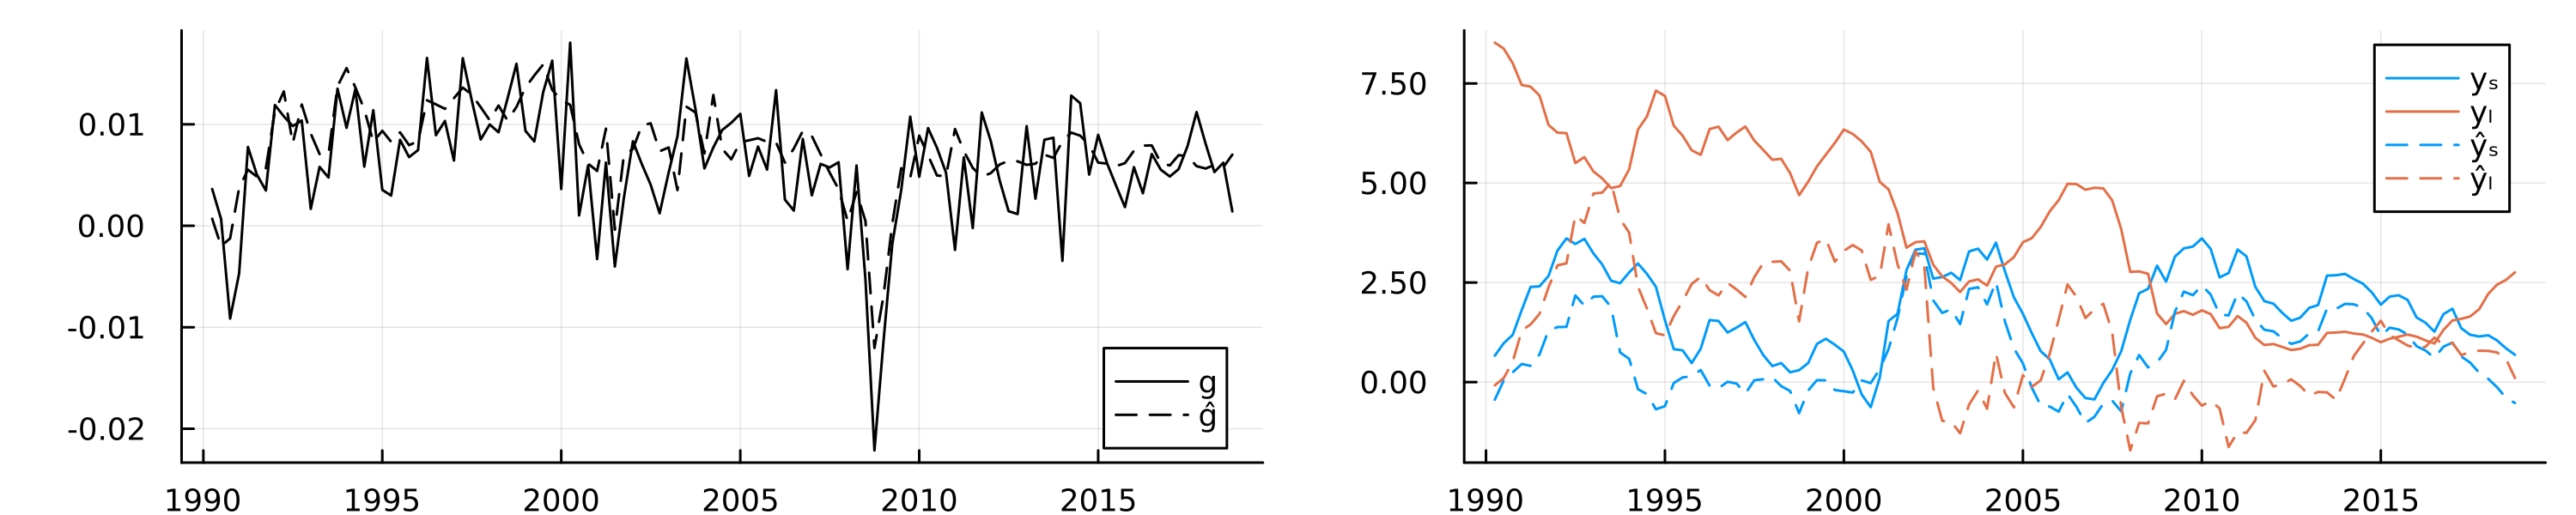
\includegraphics[width=0.8\textwidth,height=\textheight]{www/dl.png}

}

\caption{\label{fig-dl}The left chart shows the actual GDP growth and
fitted values from the autoencoder model. The right chart shows the
observed average level and spread of the yield curve (solid) along with
the predicted values (in-sample) from the linear probe based on the
latent embeddings (dashed)}

\end{figure}%
\end{frame}



\end{document}
